\chapter{Discussion}
\label{chap:discussion}

In this chapter we will provide a discussion of the findings done in the two workshops we have conducted, and on the concept we have created. We will link our findings and results with theory and previous studies, as well as provide our own opinions. The concept is developed based on findings from workshop 1, findings in related research, and official guidelines. Some of the choices made in the concept come clear from this, however, some choices were made by us with no foundation in theory. This will be discussed in Section \ref{sec:discconcept}. In the discussion of the findings from workshop 1, found in Section \ref{sec:discfindings1}, we conclude in each subsection with what was taken into consideration in the game concept. In this way, the reasons for the choices made in the concept will come clear from here. There were some topics we learned during the conduction of the research, that are out of the scope of this thesis, but that there were spend some time on, nevertheless. An example of this is the delay problem which was discussed several times with the informants. Because of the great importance of this issue, we will provide a brief discussion on this topic. However, studying this problem in depth, and finding a solution for it, will be left for future work. At last in this chapter, we discus the quality of this study.

\section{Discussion of Findings from Workshop 1}
\label{sec:discfindings1}

In Section 6.1. we discussed the importance of usability which is about how easy a system is to use, learn and understand. Workshop 1 was performed to see how a set of relevant users interacted with existing commercial exergames, and to identify which aspects of these games that do or do not work for this user group. In Section \ref{sec:usability} we present three relevant elements that can say something about a system's usability: \emph{effectiveness}, \emph{efficiency}  and \emph{satisfaction}. These were aspects among others that we tried to measure in this workshop. We also tried to answer the exergame's \emph{context of use}. We wanted to discover the needs of the intended users, the need for functionality, and the environment for the game. Where and in what circumstances the game can be used, were discussed in our previous project assignment \cite{project}. This is not our main focus in this thesis, but will briefly be discussed in Section \ref{subsec:whatwhere} for the interested reader.

In this section, we will discuss the findings from workshop 1 and relate these findings to the literature provided in precious chapters. From this we will emphasise what we have considered in the concept. With the findings from workshop 1 and the literature study conducted we have tried to answer these two research questions: 

\emph{RQ1: Are existing commercial Xbox Kinect games suitable for exercising purpose for the senior user group?}

\emph{RQ2: What are the design challenges when developing video games aimed for exercising for the senior user group?}

First, we will provide a general discussion, and then we will summarize by more precisely answer the two questions at the end of this section. 

\subsection{Control of Character, Clear Goals and Mastery}
The GameFlow model \cite{sweetser} discussed in Section \ref{sec:heur} describes eight core elements that should be present to experience enjoyment in games. One of these is \emph{control}. The informants expressed that they did not feel that they had control over their character. This was due to the significant delay that was present in the games. In addition it came clear from the observation that it was not always easy to understand when the game started and ended, as well as what was an instruction video and what was the actual game. The element \emph{clear goals} did also seem to lack in the commercial games, and it was expressed by one of the informants that there was a need for more instructions on what was actually expected from them and the rules of the game. In Section \ref{sec:sergames} we discussed how video games can function as a pedagogical tool and it was shown that important factors to focus on includes motivation, effectiveness and intuitiveness.  These aspects were also mentioned by the informants, who stated that the system needs to be easy to understand, and that the feeling of mastery and that you learn something are important.  One informant mentioned that if they did not manage to do something, they would stop doing it. In our game concept we will focus on emphasising the goals in the game, and the player will be rewarded with points. In addition we provide different levels. This will be done in two ways: Different initial difficulty levels the player can choose between, and different difficulty levels within the initial levels, where the next level depends on the previous.  

In Section \ref{sec:motivators} we discussed self-efficacy as an important determinant of exercise behaviour. Elements that are relevant to sustain this exercise behaviour are the feeling of pleasure and satisfaction, and self-regulatory skills. This was also discussed in workshop 1 as important aspects, and the informants mentioned goal setting, the possibility for socialising, and the possibility to self decide what to do, as important. The feeling of mastery was seen as significant. They were clear that if they did not get the feeling of mastery, they would not play these games. This relates to the elements discussed in the GameFlow model \cite{sweetser}, where some of the criteria for player enjoyment in games are to include challenges that match the player's skill level, to have different levels of challenges, and clear goals. Clear goals, with appropriate challenges to reach goals, are aspects highly considered in the new game concept.
 
\subsection{Immersion and Concentration}
As presented in the GameFlow model \cite{sweetser} immersion and concentration are important aspects of the gaming experience. It was hard to evaluate from observing and interviewing informants if they were immersed into the game and concentrated on the tasks. However, comments like \emph{"I felt like the person [avatar] itself"}, and cheerful comments given by the informants while they played, like \emph{"I wanted that pineapple"}, suggested that the informants immersed into the game. If we are to evaluate, we would say that all the games required concentration to perform the tasks right. However, it did not always seem like the informants were that concentrated. One example of this is that we sometimes had to assist the informants in reading messages appearing on the screen, like "raise hand above head to play", while they other times read the same type of messages themselves. We believe that the text should have been clear enough, and that the reason for them not reading the text, was because they were not concentrated enough on the game. 

Concentration and immersion are considered in the exergame concept. For the player to see obstacles on the trail, as well as see when apples get ripe, they need to concentrate. In addition, the activities are provided in a real-life environment well known for elderly, and are based on activities suggested as interesting for them, which should make it likely to immerse into the game.

\subsection{The Possibility to Customise}
As mentioned, in our previous project \cite{project} we evaluated the game to fit as a tool that physiotherapists can use as an alternative exercise method for their patients. The value proposition of this game was described as: \emph{"A tool with the ability to customize an exercise program, and to offer an alternative, fun and motivating training method, while at the same time ease the workload of the physiotherapist"} \cite{project}. In this thesis we have focused on one part, of this description: \emph{an alternative, fun and motivating training method}. For this game to meet these three criteria, the end-users had to be included in the development process. However, as learned from g.1, as well as from the informants, there is a need to customise these kind of games and acknowledge elderly's various limitations and disabilities. One example given by the informants was that the skiing game could have too fast pace for some people within this user group, and that it could cause problems for people with decline in their balance function. The possibility to customise the games can for example be a feature in the physiotherapists interface, where they can put together different exercises within the game story, that fits their patient. Another example is for the user herself to have an interface where she can put together her own program.  Requirements 1.34, 1.35, and 1.36 in Table \ref{tab:func3} in Section \ref{sec:req} are presented to meet this possibility. We have limited our thesis to not design a user-interface for this and this is therefore left for future studies. 

\subsection{Social Aspects}
The Game Flowmodel says that games should support social interaction to meet player enjoyment. Also in Section \ref{sec:exergames} the importance of social interaction in exergames are discussed, and  in \cite{statistics2012} it is stated that as much as 62 percent of all gamers say they play with others. Guideline g.8 discussed in Section \ref{sec:summaryguidelines} also suggest to including social factors in a game for elderly. Offering social interaction, can especially be important for elderly who experience loneliness in their everyday life, due to inactivity \cite{exergamesforelderly}. It was interesting to learn that social interaction also was seen as important by the informants. The majority of the informants would rather play together than alone. However, none of the informants could see themselves playing together with others over the Internet. This relates to the findings done in \cite{Gajadhar} where it was shown that elderly enjoyed playing together in the same room more than playing online. We believe that one of the reasons why the informants stated this was because they did not understand the concept of "playing over the Internet", as a result of their inexperience with this technology, which is also stated as characteristic c.7 in Section \ref{subsec:characteristics}. This might indicate that the market is too immature for this. 

One of the informants meant it was more motivating to cooperate than compete. This was also found in \cite{Gajadhar} where they in line with the result from their study and from previous studies conclude that the focus should be on cooperative play rather than competition for this group of people. This was supported by one of the informants' comment. However, the others seemed indifferent. In our game concept we will provide both the possibility to compete and collaborate, because of two reasons: First, several of the informants wanted the possibility to play with grandchildren. The findings they did in \cite{Gajadhar} about elderly preferring collaborating and helping each other, rather than competing, were in contrast to what they had found about young people in previous studies. Second, the majority of the informants were indifferent. 
 

\subsection{Appropriate and Simple Feedback and Information}
In Section \ref{sec:summaryguidelines} we listed typical characteristics of elderly based on findings from the literature. In our research we had a group of informants, who were relatively physically and mentally fit. From the list provided in Section \ref{sec:summaryguidelines}, we only experienced c.2, c.7 and c.9. We experienced that one of the informants had problems reading the text in some of the menus. Because it was only one informant that had problems with this, we assume that this informant might have had impaired vision. However, as discussed in Sections \ref{sec:summaryguidelines} and  \ref{sec:designelderly} impaired vision is a common problem for the older population, and should therefore be considered in a game designed for this group. The group of informants had interest in technology and used different types of it, like computer, tablets, mobile phones, e-mail, e-banking, TV, etc. However, none of the informants had any experience with video games. In the beginning of the workshop we experienced that some of the informants were insecure, and had problems understanding what they were suppose to do. It took some time for most of them to understand that they had to use their body to play. Therefore, we see a need for clearer instructions both before and under game play. This includes an introduction to how the system works, like how to interact with the sensor. The last of the characteristics listed in Section \ref{sec:summaryguidelines}  we experienced, was that some of the informants expressed that it was hard to do more than one thing at the same time. Therefore, the information given, and the tasks to be done, should be limited, and adjustable. The possibility to add more functionality after the existing functionalities are managed was suggested by one informant. This is also stated in g.11, and suits well with the requirements of simplicity discussed in Section \ref{sec:simplicity}. 

The last of the GameFlow elements the informants were not satisfied with was the \emph{feedback.} Number 3 and 4 of the eight golden \cite{mmi} rules presented in Section \ref{subsec:golden} discuss the importance of getting informative feedback at appropriate time, and guideline g.6 presented in Section \ref{sec:summaryguidelines} suggest that feedback should be given in a motivating form. The informants desired more feedback on their actions, and they especially wanted to know whether they did the exercises right or wrong. They did not feel that they got this feedback in the games played in the workshop, which made them both confused and frustrated at times. Some of the games that were played had a lot of different features that were suppose to be motivating. However, by some of the informants this was rather seen as annoying.  In addition the amount of the information given, both text and audio, was experienced as too much. At the same time, some of the informants stated that they did not recognise these type of messages at all. In Section \ref{sec:simplicity} we discussed minimalistic design which is about bringing the most important elements into focus, without elements that will distract the user. Microsoft presents it as "Simple Can Be Powerful", which means that simplistic design not necessarily needs to mean lack of functionality. From this we conclude that we should avoid too much features in our video game concept. We should keep it simple, and focus on a few motivating aspects. One of the informants desired more time to read information and instructions, and suggested that there should be a way to tell the system when you are finished reading. This is supported by guideline o.22 in Section \ref{sec:designelderly}, and will be taken into consideration in our exergame concept. 

\subsection{Cultural and Lifestyle Diversity}
Guideline g.7 presented in Section \ref{sec:summaryguidelines}, and e.2 presented in Section \ref{subsec:golden}, are about matching cultural and lifestyle diversity in the games. This was expressed by the informants as important, and they suggested different type of themes for a possible game concept, like dance, swimming, apple picking etc.. If they were to play a game like this they stated that it would need to include sports or activities related to real life. They also mentioned the importance of appropriate music. They did not like the music in the commercial games because they were not the type of music they used to listen to. M.13 presented in Section \ref{sec:motivators} propose appropriate music to be a motivator for exercising, and \cite{schutzer} sees music also as a way to divert from pain coming from the exercises. The majority of the informants agreed that music was important, especially to keep the rhythm. However, they stated that they wanted it quiet, and they wanted music more related to their generation. This indicates that choosing the right music is an important requirement that should be set for the exergame, however, it is outside our profession to come up with specifics about what music to include. 

The informants' opinions did not differ much according to gender on what they liked and did not like in the games we tested. However, as discussed in Section \ref{sec:motivators}, different people's needs and expectations, as well as aspects such as gender and ethnicity should be considered. We will meet this by creating a concept with a series of games that covers a variety of interests, as well as getting to choose a male or female character. Race might also be considered, but it is difficult to cover all races. Chao et al. \cite{chao} discuss that to meet diversity requirements, it is important to be in contact with the relevant people. Even though we clearly have not covered the total group of elderly, we have included a small group to understand some needs and expectations.

\subsection{Summary}
We will now provide a summary of the discussion to in a more precise way answer research questions 1 and 2. 

In our previous project \cite{project} we discussed that the existing commercial games are not aimed for the elderly user group, as they are too rapid and complicated. In the several related research presented in Section \ref{sec:relatedresearch} this was seen, and different characteristics of elderly were discussed, and guidelines were suggested. We wanted to explore this closer, by testing different types of games to see what are good and bad aspects with the existing games. Findings from this together with the previous research will answer research question 1:

\emph{RQ1: Are existing commercial Xbox Kinect games suitable for exercising purpose for the senior user group?}

As mentioned initially, effectiveness, efficiency  and satisfaction are relevant measurements when evaluating the usability of systems. From findings done in workshop 1 we can conclude the following about the commercial games tested: 
\begin{itemize}
\renewcommand{\labelitemi}{$\bullet$}
\item The existing commercial games tested on a group of elderly do not meet the requirements of effectiveness. The games do not spend enough time on instructions and information, and do not give sufficient feedback on what the players are doing is right. The menus are too complicated and it is too many elements showing at the same time. The buttons presented in the games are too sensitive, and it is not intuitive how to press the buttons. 
\item The existing games meet only to a degree the requirement of efficiency. In FruitNinja it was clear that the informants did not understand what was required from them, and they just waved their hands uncontrollably. The majority of the the informants understood what was expected from them in the tennis game, and played through this game without problems. The skiing game was also well understood, until the second match where the two players that played together switched tracks. All of the informants had problems relating to their player after switching tracks. None of the menus met the requirements of efficiency. We had to assist the informants through the menus, and because of too much information and too sensitive buttons, the informants spend unnecessary time on getting through the menus.
\item Two of the four games played in workshop 1 meet the requirement of satisfaction. All of the informants liked playing the tennis and skiing game and they had fun while playing. FruitNinja, they did not like that much, which relates to their wish for playing games with a meaningful content that they could relate to everyday life, which is not the case for FruitNinja. The informants were not satisfied with the personal trainer game either, because this focused on "just" regular training, which they would rather do without the game. This strengthens up under Michael Zyda's statement on that the main focus in serious games should be on fun and entertainment \cite{zyda2005visual}. 
\end{itemize}

It is important to remember that this was the first time the informants played games like these, and initially they did only play the games once \footnote{Three of the informants got to play the skiing game a second time because they specifically asked for it. We did not observe anything new in this second session, and have because of this, and because the rest of the informants did not try a second time, not included this in our analysis}, which did not enable us to say anything about the informants learning curve. However, we did see that they understood more what was expected from them, and that they got more confident after a while. If we had went on with several rounds with the same games, we might have seen improvements. This was also mentioned by the informants. 

From research and workshop 1 we have also looked for answers to research question 2. This is to make it easier to know what to focus on when developing a exergame for the senior user group.

\emph{RQ2: What are the design challenges when developing video games aimed for exercising for the senior user group?}

One of the main challenges developing an exergame for this user group, is that they are a group with diversity both when it comes to interests and different type of disabilities. Different characteristics of elderly are listed in Section \ref{subsec:characteristics}. These should be taken into account when developing for this group. Our informants desired a game with a story that appeals and relates to real life, as well as appropriate music to their age. Different themes for a possible game were mentioned, showing the diversity of needs. The game should meet the requirements from the GameFlow model \cite{sweetser} that we discussed to be important in Section \ref{sec:heur}. We found this model to serve as good guidelines, as many of them was mentioned as important aspects by the informants, and also because there is a clear relation between these guidelines and the guidelines we can draw out from the literature, presented in the previous chapters. It was urged for more instructions on how to interact with the game, as well as what was expected from the players, the goals, and the rewards. The menus in the commercial games were seen as challenging because of the amount of information and the sensitive buttons. In a game for this user group this needs to be improved, taking physical disabilities in arms and visual decline into consideration. The majority of the informants would only play these type of games together with others. Guideline g.8 presents social aspects as important, as well as it is a recommended guideline in the Game Flow model \cite{sweetser}. Therefore, it is important to include this in our game concept. The delay in the games was seen as a big problem, and should be acknowledged.  This is a technical issue that we are not in the position to evaluate the reason for. We believe that if this game is to be used for exercising, both at home and in clinical settings, technical precision have to be present. 

\section{Discussion of the Concept}
\label{sec:discconcept}
The idea for our concept is not random. It is well thought through, founded on background theory and our own findings. However, some of the choices made do differ from the findings. For example o.18 presented in Section \ref{sec:designelderly} is about the importance of using a one-coloured background, as well as not having text on pictures. We chose to have transparent text-boxes in front of the pictures when giving information and instructions. We chose this to not interrupt with the picture of the game environment. Having the box filled with colors hides too much of the picture, and it does not look very nice. In this case, we chose design over usability. However, o.18 also says that the text should be put where there are light areas in the picture, which wee meet by putting black text over a white transparent box.    

A limitation of the presentation of our exergame concept is that we do only....SE HER

boss

\section{Discussion of Findings from Workshop 2}
\label{sec:discfindings2}
In Section \ref{sec:userinvolvement} we presented how important user involvement is during system development, as the end-users are the ones who will use the final product, and are the only ones who know what they want. After making a concept based on specified requirements, we wanted to invite elderly to a second workshop to get feedback on our ideas and design proposals. In workshop 2, we presented our prototypes for an exergame concept for a group of elderly, and we opened up for questions and discussions. Figure \ref{userdesign} shows the cycle for user centered design, where workshop 2 is about the fourth step, evaluating system design up against usability. As presented in Section \ref{sec:userinvolvement}, ISO 9241-210, states that feedback from users will help designers not only evaluate design, but also improve them according to the users needs. Involving the end-user in the design process will increase the possibility of making a user-friendly interface for the intended user group, which is, as stated in Section \ref{sec:usability}, crucial for making a successful system. 

In this section feedback from workshop 2 will be discussed, and we will present important aspects to be included in the future work of designing an exergame for elderly. These aspects will only be discussed, we will not make any changes to our current exergame concept, as this is out of the scope of this thesis. Our findings from workshop 2 will be related to theory provided in previous chapters.

\subsection{Few Comments and Moderate Response}
Generally there were few comments, but several questions, during the workshop. When we presented the various prototypes, the informants responded with silent nodding or just looking mutely at the screen. There could be several reasons for this. One reason could be because the informants were inexperience with video game technology, which could have made it difficult for them to comment on a video game concept, as they did not know what to look for and respond to. One informant stated that it was impossible for her to comment on our exergame concept, as she did not know anything about how the game would work. Another reason could be related to how we presented our prototypes. Our exergame concept is based on highly interactive video game technology, and as presented in \ref{sec:prototypes}, this is very difficult to make good prototypes for. In addition, the Kinect technology do not use any sort of controllers that we could have made prototypes for. When we made our prototypes, we made them with the purpose of showing various scenarios from the game. We did not make our prototypes in a way where it was possible for the informants to interact with them. We presented the prototypes with the "Wizard of Oz", meaning that one of us controlled the interactive system, and the other one took the role as the user. This was to try to give the informants a feeling of interaction. However, the lack of interaction between the informants and the prototype could have been a reason for the informants poor understanding of how the game would work. 

A final reason could be that we did not present the information good enough. A question from one informant supports this assumption. She asked if the avatar in the prototype would respond to her movements, even though she had played games like this before. After we explained the relationship between the avatar and the player, it seemed that the informants understood quickly. This increased understanding lead to more questions and feedback. Also, it became clear that it was not clear how the quizzes would appear. I4 thought the quizzes had to be answered at the same time as doing other tasks. She suggested that the quizzes should be separated from the other tasks. This was the way we initially had thought it to be. This misunderstanding was a result of us not presenting this clear enough.

\subsection{Challenge, Concentration and Difficulty Levels}

The GameFlow model with its concentration element, emphasises the importance of not distracting players from tasks they want or need to concentrate on. In addition, players should not be bothered with tasks they see as unimportant. Related to this concentration element, the informants had some concerns and uncertainties about integrating quizzes in the trail. The informants expressed that they felt that having quizzes together with physical tasks would draw attention away from one of the them. They did not like the idea of doing two thing as the same time. \emph{"I would like to focus on the task I am supposed to do"}, one of the informants said. It is important to take the element of concentration into consideration when developing an exergame for elderly. Characteristic c.9 says that elderly has difficulties doing more than one thing at the same time. We suggest that one solution for future work could be to choose, when starting up the game, whether you want to include the cognitive challenges or not. 

One informant suggested that the quizzes should provide different categories, to meet different interests and knowledge areas. On the work on the concept, we have not focused on what kind of questions that will appear, we only provided an example question. Further work should include finding an appropriate way to engage cognitive skills and to find suitable questions and tasks for this.

From the challenge element in the GameFlow model we know that games should offer difficulty levels that matches the player's skills. This, combined with the concentration element, have lead to the idea of adjusting frequency between the appearance of obstacles and number of simultaneous tasks according to the various difficulty levels. The difficulty of required exercises and movement should, in line with guideline g.11 and g.12, also be controlled by the difficulty level, as this is an important feature for elderly that might suffer from various physical challenges. One informant stated that balancing over a log looked challenging, as she though she would feel dizzy, and that she was afraid of falling in real-life. This challenge was also reviewed by a physiotherapist. She stated that it was a difficult exercise to perform, and therefore should be included in higher levels in the game. This support the importance of providing the possibility for players to choose difficulty levels themselves, like stated in guideline g.13. However, the GameFlow model emphasises that the game also should support adjustment of difficult level after the player's skills and progress. By offering both these opportunities in this exergame, we meet the feedback from the informants, as they want to be able to master the various tasks, and not be forced into something they would not master. They both wanted to choose themselves, and to let the game follow their increased skills, so they could feel that they learned something and got better.  

\subsection{Graphics, Sounds and Interface}

Feedback shows that the informants liked the exergame concept we presented for them. The informants expressed that the concept with the nature trail was a good idea because they were familiar with the environment. This supports findings from previous studies, like in \cite{gerling2}, where the participants appreciated the use of a real-life environment. The GameFlow model states that immersion is important for the player to effortless be involved in the game \cite{sweetser}, and we believe that the use of an natural and real-life environment can be helpful for achieving this engagement. 

Guideline g.4 and o.8 emphasise that an interface should be simple and not to complex, and that important elements should be brought into focus. The informants seemed to like and understand the menu interface we presented for them. Their general perception of the interface was that is was \emph{"beautiful"}. The back-button and the purpose of it was observed and understood immediately. A comment was to highlight the buttons even more, making them stand out more with a hint of shadow around them. 

SilverPromenade, presented in Section \ref{sec:relatedresearch}, had success with an intuitive and user-friendly interface, which quickly and easily guided the users to game play. However, as mentioned in \ref{sec:menu}, we have chosen a to have a longer menu to include the possibility to choose actions, and at the same time avoid too much information at each step. The informants felt the menu was OK, but they wanted to use shortcuts when they had got familiar with the game. Inclusion of shortcuts for the experienced user is mentioned as an important feature in the second and seventh Golden Rule, presented in \ref{subsec:golden}, and should therefore be included in future work for this exergame.

Generally, there were a lot of questions related to various elements in the prototypes. An example was a question about what the hearts meant, and what would happen if the player touched them. That the hearts were observed quickly is positive, as these are important elements of the game. This means that they stand out, which is stated as important. However, from the last of the Eight Golden Rules, we know that intuitive interfaces also are stated as important. What is not so positive with all the questions, is that it shows that our interfaces are not that intuitive as we had imagined them to be. This has to be taken into consideration for future work. We also got questions and feedback that indicates that there were to much elements in the picture. In our prototypes we have shown obstacles, hearts and quizzes all in the same picture, and we presented it this way to show how elements will appear along the way in the nature trail. However, the informants did not see the depth in the picture, and believed that they were suppose to do everything at the same time. This made the prototype appear quite distracting, as the informants did not know what to focus on. This interferes with the concentration element, therefore, presentation of elements has to be considered in future work. 

Two elements in the menu were a source to a lot of discussion due to lack of intuitiveness and consistency. One of these was where the player was to choose environment and difficulty level. This especially yielded the understanding of the increased difficulty level between the three environments. It came clear to us that it was not very intuitive that the three different forest environments we presented were meant as three different difficulty levels. Future work would be to focus on including textual information to make this part more intuitive. A suggestion would also be to have instructions on what different difficulty level implies and means. The other menu step was where the player had to chose to play according to a specific muscle group. The informants did not see consistency between the term "muscle group" and what we presented in the menu. I1 said \emph{"The term muscle group, it does not fit with what you show here [...]"}. This is not positive for our interface, as the first of the Eight Golden states that designers has to strive for consistency to achieve good system design. We acknowledge that we did not think through this step thoroughly. However, what we presented was just an example, and we concluded that it is future work for professionals, like physiotherapists, to find appropriate muscle groups to include in the exergame.

As a motivator for exercising discussed in Section \ref{sec:motivators} and \ref{sec:georep}, we know that sound and music are important for the players enjoyment and gaming experience. We did not present any music, or soundtrack, for the elderly, as this, as mentioned in Section \ref{sec:outinthenature}, is out of our competence area. However, we told the informants that we wanted to use calm and peaceful music, to meet their feedback from workshop 1, where they expressed that it was too much noise. We also presented the informants for ambient effects, like birdsong and sound of running water, as this are sounds related to the environment of the game, and sound effects like a "ping" when collecting a heart. They seemed OK with this music and sound, but they wanted music with more rhythm to easily immerse into the game and exercise. Future work would therefore be to find appropriate music for the nature trail and the single games, based on the exercise and pace in each game. 

The informants had questions about what would happen if they were to fall down from the log and into the river. Technical issues similar to this question could include the possibility to walk outside the path and into the forest. We had not included these kind of technical limitation in the system requirements because we simply did not think about it. Because we are familiar with computer and video games it is obvious for us that there are limitations to avoid the player from "walking our of the game world". However, this is not necessarily obvious for the user group. These kind of limitations are aspect that needs to be looked further into and integrated into the system requirements.

\subsection{Summary}
\label{sec:summarydiscW2}
We will now provide a summary of the discussion of findings from workshop 2, where we will draw important aspects to consider in the future work of the developing this exergame for elderly. 

\textbf{Future Work for an Exergame for Elderly}
\begin{itemize}
\renewcommand{\labelitemi}{$\bullet$}
\item Future work should include working on how to present the idea of difficulty levels for the users. There should be focus on including instructions and information about how difficulty levels are chosen and controlled. In addition, textual information should be included in the menu step where the player is to choose environment, to indicate that each environment holds initial different difficulty levels.  
\item Our prototypes showed obstacles, hearts and quiz icons all in the same picture, which made the prototypes distracting. Future work should include studying the presentation of elements. A suggestion could be to not show the elements from a long distance, but let them appear as the player comes closer to them. 
\item In future work, the exergame should hold the possibility to separate the quiz from the nature trail. This should be done to let the player more easily focus on one task at the time. It might be more natural to include the quiz when the player has gotten more familiar with the game.
\item Future work should focus on how the quizzes should work, and how and when they will appear. We observed a clear need for a thorough introduction on how the quizzes will work. Future work could also include looking into presenting the quiz icons in a different way, to not take focus away from the other current tasks. 
\item The buttons in the menu should be highlighted to let them stand more out. This can be done by adding some shadow around the buttons.
\item Appropriate shortcuts should be included in the menu. These should not interfere with the functionality already provided by the Kinect, like pausing by holding the left arm out from the body.
\item It should be the future work for professionals to find appropriate music to the game. This yield ambient effects that fit the environment, sound effects to give users feedback on actions, like when collecting a heart, and music suitable for the intensity in the game.  
\item It is important to include the purpose of all important elements in the instruction video. The idea is that the purpose of the hearts, and all the other elements, shall be presented in an instruction, but this was not included in our presentation. We observed how the lack of instruction created confusion, and we therefore see the importance of having these instructions.  
\item It should be the future work for professionals, like physiotherapists, to find out which muscle groups to present as choices when the player wants to play according to a specific muscle group. Our lack of knowledge in this area shone through when we presented this part, as the informants quickly commented the lack of consistency between the term "muscle group" and what we had presented as muscle groups to choose from. 
\item Technical limitations should be explored and integrated into the system requirements.
\end{itemize}

\section{Challenges Related to User Involvement}

It is important that we acknowledge the difficulties about engaging a user group into a setting they are completely unfamiliar with. It is hard to evaluate some users needs, when they do not even know about these needs themselves. We have learned from our two workshops and our previous project \cite{project} that today's elderly are not necessarily the right user group for a game like this, but that the next generation of elderly might be more suitable, because they are more familiar with the use of technology in their everyday life. However, it is hard to test a tool that is meant as an alternative form for exercising on people who are physically in good shape, and who keep one doing regular exercising. Therefore, a group of today's elderly was included.

Most elderly are inexperienced with video game technology, and it could be difficult to include them in a development process for an exergame, which is completely new for them, as well as something they have not acknowledged the need for. We found it challenging to include such an inexperienced user group in an early development phase. This it not just based on the development being in an early stage, but more the fact that elderly are very inexperienced and unfamiliar with the video game technology Kinect provides. The elderly did not know what to look for or respond to when prototypes were shown to them, as they had problems relating to what we presented. We believe that this could be a reason for not getting that much feedback on our prototypes. However, it could also be a result of how we presented our prototypes. It is difficult to make interactive prototypes for such a complex and interactive system. We know from Section \ref{sec:prototypes}, that how users interact with the prototype is crucial for understanding the system. It was not possible for the informants to interact with our prototypes, which might have lead to lack of understanding. It was not easy for the inexperienced informants to come with feedback on such an interactive system, when they were presented for still pictures, even though they had played Kinect games in workshop 1. We believe that a more interactive prototype would have lead to more understanding and that it would have triggered more feedback. Interactive prototypes would make it possible for the users to try to play, which would make it easier for them to understand how the game would work. This should be provided in a next phase of the testing and evaluation of this game concept. However, this is out of scope of this thesis.  
 
 
\section{The Delay Problem}
\label{sec:delay}
Both in workshop 1 and workshop 2, there were a lot of time spent discussing and commenting technical aspects related to the delay between the player and the avatar on the screen. This problem was a source to much confusion and frustration, and it did not give the informants a real-time experience. The informants also stated that the delay ruined the overall gaming experience. It is obviously crucial to take this into consideration when developing an exergame, as the delay partly destroyed enjoyment and immersion when playing. The control element in the GameFlow model \cite{sweetser} is about the player being in control of their actions, characters and movements. Feedback from the two workshops were that the informants did not felt this control, due to the delay. \emph{"There was no relation between our own movements and actions on the screen"}. For an exergame to be accepted and used in physiotherapy clinics or training groups, there has to be done something with this delay. 

When searching Google for "Kinect" together with "delay" or "lag", we got a lot of results, both articles, and forum questions and discussion. This can indicate that we are not the only ones who have experienced problems with Kinect's real-time presentation. We wanted to play some games over again to see if the delay was still there, or if it was just a one-time coincident. We started by playing the "Your Shape Fitness Evolved 2012", where we chose to play the same game as we presented for the informants in workshop 1, the Humana game "Aging with Grace". This is shown in Figure \ref{fig:remakeDelay}. Observing this figure, we clearly see that there is a significant delay between the players movements and the avatar on the screen. The avatar to the left is the trainer, while the other avatar portrays the player. What we can see here is that the player is following the trainer's movement, having the arms down, while the avatar portraying the player are behind, having the arms straight out to the sides.

\begin{figure} [H]
\centering
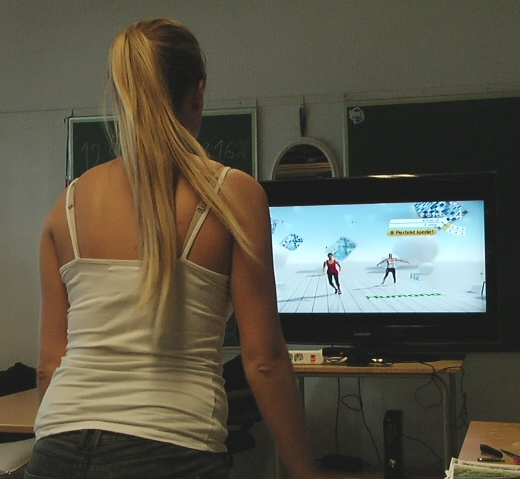
\includegraphics[scale=0.6]{kineDelay.jpg}
\caption[Kinect sensor delay]{This figure shows that there is a clear delay between the players movements and the avatar on the screen.}
\label{fig:remakeDelay}
\end{figure} 

We also tried "Fruit Ninja" over again. [HER SÅ VI IKKE LIKE TYDELIG DELAY].

We noticed that a clear difference between the "Your Shape Fitness Evolved 2012" and "Fruit Ninja" is the amount of information being processed. In the personal trainer game, the player's movements are tracked and compared to the required movements, and based on that, precision and various variables, like calories burned, are calculated. These calculations are not present in "Fruit Ninja". As these calculations are both process and time consuming, we believe that it is a source to the experienced delay. Our assumptions are supported by various articles, like \cite{kinectLag}, where it is stated that fitness games that uses skeletal systems requires more time to calculate than other games, and that these games normally experience delay. 

From a review done on some of forums found when searching Google, it seems like the degree of delay varies within different games. It is clear that people have different opinions about Kinect and the delay problem. Some people do not notice the delay at all, while others feel that Kinect is not nearly as good as its reputation, due to the delay \cite{kinectLagForum1} \cite{kinectLagForum2}. \cite{kinectLag} may support the assumption about delay depending on the game played. Here, Andrew Oliver from Blitz Games, states that software could be the source to the delay, and that the delay can be eliminated if developers choose the right software to build their game upon. Shotton et al. have written a paper where they present a method for giving quick and accurate prediction of 3D positions for Kinect. By learning the Kinect software how to predict human movement and behaviour patterns, process speed can be increased while delay is increased \cite{artikkelKinectLag} \cite{artikkelKinectLagIntro}. This paper gives a detailed presentation on how this could be done, and we refer the interested reader to \cite{artikkelKinectLag}.       

\section{Miscellaneous Aspects to Consider About the Exergame Concept}
\label{sec:misc}

\subsection{Discussion on where and in what circumstances the game can be used}
DENNE ER IKKE FERDIG, MEN SKAL SNAKKES LITT MER OM.
\label{subsec:whatwhere}

In our previous project \cite{project} we evaluated the game to have the most potential in a clinical setting, offered as a training method at physiotherapy clinics. This was based on two main things. First, "Samhandlingsreformen" encourage the use of welfare technology where possible in health care. Second, the majority of the senior user group, have little or no experience with video games, which will make it hard to reach out to these customers. In this thesis we have not focused on where the game should be implemented. However, we did ask the informants where they could see the game be used and two main settings were mentioned: in a group setting, for example in nursing homes, and in a setting with grandchildren. We decided to not study any further where the game can be implemented. This was both because we experienced that the majority of the informants had a hard time picturing themselves own and use a game like this, and also because from what we learned from the interviews conducted in our previous project, where physiotherapists could not say anything about whether they would use this game or not before they could test the actual game. For more discussion around where the game could fit, we will direct the reader to \cite{project}, and in particular Section 8.2 and Chapter 9 in that report. 

In Section \ref{sec:barriers} we discussed some challenges when it comes to motivating elderly to exercise. Some of these challenges were also mentioned by the informants. One informant saw it as a barrier to exercise if she lived far away from the training centres, and could see that the game could have a potential as a replacement for going to the gym. Another informant did not want to get controlled by time and appointments, which suggest that an exergame could be an alternative way to exercise on their own time. 
- Kommentar til avsnittet over: Fokusere det litt bort fra "oppsummering" av findings, og mer mot hva vi tenker. Som - i fremtiden, gjøre det mer tilgjengelig. Et slikt spill - få det hjem, trene på egen tid og premisser osvosv. 


- Nevne dette som skjer i Trondheim kommune, det at hjemmehjelpere tar med spill hjem til eldre. 

\subsection{Non-functional requirements not included in the game concept}



Dette er inkludert i diskusjon og ikke i konsept, fordi vi ikke har nok kunnskap til å være nok spesifikke på disse kravene. 

\begin{table} [H]
\label{tab:nfunc2}
\centering
\begin{tabular}{|l|l|}
\hline
3.1 & The system shall be able to run on both PC and Xbox. \\ \hline
3.2 & The system shall be easy to set up (physically).\\ \hline
3.3 & The system shall include Kinect functionality, like pausing \\ & a game by holding one arm out from the body. \\ \hline
3.4 & The system shall load within few seconds.\\ \hline
3.5 & The system shall be small in size and do not require too \\&  much space.\\ \hline
3.6 & The system shall not require too much capacity. It shall \\ & be able to run on a regular PC. \\ \hline
3.7 & The system shall not require too much power. \\ \hline
3.8 & The system shall avoid delay between the player's \\ & movement and action on the screen.\\ \hline
3.9 & The system shall ensure secure storage and sharing of \\ & profiles. \\ \hline
\end{tabular}
\caption[Miscellaneous non-functional requirements]{Miscellaneous non-functional requirements}
\end{table} 

\section{Quality of the Gathered Information}
\label{sec:discQuality}

Section \ref{sec:qualityresearch} states the importance of evaluating quality of the research we have done. This can be done by looking into the three criteria, \emph{reliability}, \emph{validity} and \emph{generalizability}. Based on this, we will discuss each criteria up against our work in this thesis. In addition, we will discuss some pitfalls that we might have experienced during our qualitative research.  

\subsection{Reliability}
It has been important in our thesis to distinguish between our own findings, and findings from theory and previous studies conducted by others. Our findings are presented in chapters separate from theory and literature, see Chapter \ref{chap:findW1} and \ref{chap:findW2}. In these chapters, neither our own opinions or theory are included. These chapters only emphasise feedback and opinions from the informants, where feedback are written as summary of discussion, or as direct citation. Findings from the two workshops are related to relevant theory in our concept chapter, Chapter \ref{chap:concept}, and in our discussion in this chapter. This separation of information will strengthen the reliability of the information gathered.

The sample of informants chosen for our qualitative research might have affected the quality of our study. Our chosen informants are all members of "Seniornett", and are elderly that are very committed to learning technology. All of them already use a wide range of technology devices, as mobile devices, tablets, and computers. We see them as more experienced with technology than most elderly in the same age group. Most of the informants have a high education, and they are relatively active in their everyday life. Five out of seven informants stated that they are active in the means of exercise, while the two others mentioned that they are active due to everyday tasks. We will state these informants as fit older people. The informants average age in workshop 1 were 70.6 years (with a standard deviation of 7,9 years), and 74,5 years (with a standard deviation of 7,5 years) in workshop 2. We feel that these informants are representative for our qualitative research based on their age span, however, they do not meet all the characteristics that are common for the older group. These informants are a group of fit elderly, and we want the exergame to also be accessible for both frail, disabled and inactive older people. This is a group of people might have experienced reduction in functionality, which make it difficult to perform regular exercise and everyday tasks, or they might just be lazy. They are in the need of a tool that can help and motivate them to exercise. However, the exergame is also meant for fit elderly that wants to stay in shape, get feedback on exercises, and have an alternative to regular exercise. 

[SI NOE OM g.14]

Our relationship with the informants is an important aspects when discussion reliability. With the exception of one informant, we had never met the informants before. The one informant we had been in touch with was the manager of "Seniornett", when he helped us to set up meetings and getting in contact with seniors. In addition, non of the informants knew each other. The fact that we were unknown for the informants could have resulted in the informants not daring to say what the actually meant and felt. It might also be the case that this sat a kind of barrier, making it intimidation talking to us. However, when first meeting the informants, we welcomed them and talked about familiar everyday topics, just making conversation. We felt this helped establish a sort of comfort. Our observation during the workshop, showed no sort of discomfort. They talked, laughed and joked a lot, both with us and each other, and we felt that the atmosphere was good. 

Our role in this workshop might have affected the reliability of our findings. What is preferred is that our participation would have been neutral, but that was not the case. We participated in the workshop by informing about the technology, showing how the different games would work, we guided the informants when needed, and we partly participated in the discussion. This might have influenced the feedback from the informants. In addition, in workshop 2, we presented a design and concept that we had made. We wished for a valuable brainstorming around the concept, and urged the informants to be critical and come with both positive and negative comments. The informants were polite, and where mostly positive what we presented. I1 said \emph{"No, it is nothing negative"} about our concept. The fact that we presented our own concept, may have lead to the informants being afraid of hurting our feelings by saying what they actually meant. 


\subsection{Validity}

In our discussion we have related findings from the qualitative research with theory and previous studies within the same subject, and what we see is that our results support what is found in this related theory and findings. We did not experience much deviation in our findings from findings in previous studies. The only aspect we can comment on, is clear interest, and questions from the informants, related to various technical aspects. The findings we got from the two conducted workshops covers a wide range of topics related to our master thesis, and they form a thorough basis for answering our research questions. We will therefore state that our findings are valid and of relevance to the purpose of the study. 

We had some difficulties placing our qualitative research method within a specific research method. Overall, our research included use of different research methods, which made it difficult to put one descriptive "title" on which research method we have used. In addition, we have used observation as a part of our overall research, which is about observing participants in a natural environment. However, this was not the case in our research, as playing Xbox Kinect games are not familiar to elderly. We tried to use an environment that was as realistic as possible, as "Gulhuset" is a place where elderly use to meet, and we imagine that to be a place where a future exergame could be used. We have, in Chapter \ref{chap:metode}, presented the research methods we have used. We have in the same chapter discussed and explained the reason for why we have chosen the various methods. We ended up describing our overall qualitative research as \emph{experimental simulation}, which is about observing people in a fixed, but as natural and familiar setting as possible. We feel that our discussion is thorough, and that it strengthen the validity of the information gathered. 
    
\subsection{Generalizability}    
Our focus in this thesis has been to develop an exergame concept for elderly. We have studied how elderly interact with commercial video games, with a goal of explore what aspects that are important to consider when developing a game for this user group. In addition, we have studied their attitudes towards exercising, and technology in general. This, together with theory and related literature, are used to specify system requirements for a video game for elderly, where our exergame concept is based on these requirements. We feel that these system requirements are so general, and are based on such thorough research, that it could be used as guidelines for others who want to develop video games for elderly. This also includes use for other cases than the one we have studied. About generalizability, Section \ref{sec:qualityresearch} mentions three types, naturalistic, moderate, and conceptual. Based on this discussion, we see conceptual generalizability as relevant for our thesis.    


\subsection{Other Quality Aspects to Consider}

In our qualitative interviews we have used focus groups as setting. Section \ref{sec:qualitativeInterviews} states that a preferred size for a focus group is 6-12 participants, but that mini-focus group interviews with 3-4 participants are accepted if the participants are experts on the discussed topic. Totally, we had seven informants for workshop 1, but these were divided into two days, with three and four informants each day. Theoretically, this means that we conducted mini-focus group interviews. The problem with that was that the informants were far from being experts on the topic, as they in fact never before had seen the technology we presented for them. However, what was a bit different with this first workshop was that the we, in beforehand of the focus group interview, had introduced the informants for the Xbox Kinect technology. We asked about their perceived gaming experience in the interview, and felt that we received good, detailed and descriptive answers. 

In the second workshop we involved five informants, where one informant that did not participate in workshop 1. That means that she attended workshop 2 with no previous experience with the Xbox Kinect technology, except from what we presented during our first meeting with "Seniornett". This made it difficult for her to relate to and understand what we presented during workshop 2, and she was therefore not able to provide us with much feedback. This is negative for the quality of the information gathered at workshop 2, as the number of involved informants already was less than what is preferred. 

In \ref{sec:otherQualityAspects} we present \emph{elite bias}, which is a pitfall that might have affected our results. Including only one group of people in qualitative interviews can give incomplete and under-representative data, and as a result, it could be hard to understand the broader situation. Because of the overall time limit for this master thesis, and other practical reasons, we only included this one group of people, even though they have the same interests for learning technology. Our data gathering would probably been different if we had gathered a group of "random" people, because they would have different backgrounds and interests.

Another pitfall, presented in \ref{sec:otherQualityAspects}, that we might have experienced  is the \emph{Hawthorn effect}. This is about observation and the risk of having people behaving differently because they know they are being observed. This may have been an issue in our qualitative research, since the Hawthorn effect may have an even bigger impact with the use of video recording. However, we tried to make a comfortable setting, and to "hide" the video recording equipments as much as possible. The informants seemed calm and unaffected by the video recording, and we therefore conclude that the Hawthorn effect did not affect the quality of our work. 

In the beginning of workshop 1, we had a presentation where we told the informants about the goal for our master thesis, the agenda for the workshop, and what we wanted to figure out and explore during the workshop. We also informed them about the technology used and the games they were about to play. About providing the informants with that much information, Section \ref{sec:ethicalchallenges} presents that participants with insight into what the researcher is looking for, might behave according to that information. This might have been the case in our workshop, as we described quite detailed what we were looking for. This could have set some boundaries related to creative thinking and what they felt was appropriate feedback. However, we felt that a thorough introduction was necessary when including a group of people with such an inexperience with video game technology. 

We will short list some additional quality aspects: 
\begin{itemize}
\renewcommand{\labelitemi}{$\bullet$}
\item User involvement is about involving users from the start to the end of the system development process. We only included the informants two times in the development process, to discover their needs and opinions, and to evaluate our design. Basically, due to the theory of user centered design the informants should have been more involved. However, this was not done due to time constraints in this master thesis, and due to the informants inexperience with technology. 
\item Workshop 1 was held over two days, but it was not executed exactly equally the two days. One day the informants got a little more instruction and guidance than the next day, some informants got to play longer than others, and not all the same questions were asked during the discussion. All this can have affected the findings from this workshop. 
\item The informants assumptions of what the workshop would involve could have affected the outcome of the workshop. 
\item Since we performed focus group interviews, the informants were influenced by each other statements and opinions. They discussed an unfamiliar topic, and it seemed easy to just "mean the same" as the informant stating something. As we had two groups of informants, the informants in within each groups formed similar opinions, that not necessary was the same in the two groups.   
\item Our choice of games that we presented for the informants was not a coincidence. Each game were chosen for a reason, which can be read in Section \ref{sec:chosengames}, and we wanted to trig different reactions. This could have affected the outcome of our qualitative research. Choosing different games might have changed the findings from our research. 
\end{itemize}

\subsection{Our Conclusion}

